Рекомендательные системы --- компьютерные программы, используемые в попытке предсказать какому объекту пользователь отдаст своё предпочтение или какой "рейтинг"\space поставит.
Эти системы персонализируют наше взаимодействие с сетью, подсказывая что посмотреть, что купить, что послушать, с кем подружиться, что почитать и т.д. Для этого они анализируют наше взаимодействие с различными сервисами и выделяют шаблоны поведения, а также объекты, с которыми мы взаимодействуем.
Существенным для рекомендательных систем является накопление знаний об активности пользователей или свойствах объектов.
Самые базовые имплементации основываются на предположении о том, что людям понравятся вещи, похожие на те, что им уже нравятся, а также вещи, которые нравятся людям с похожим вкусом.

Рекомендательные системы можно разбить на 3 категории:
\begin{itemize}
\item На основе содержимого --- модель, которая использует множество свойств объекта для рекомендации объектов с похожими характеристиками;
\item На основе коллаборативной фильтрации --- модель, которая учитывает историю взаимодействия пользователя с сервисом (купленные товары, прослушанная музыка и т.п.), а также поведение похожих пользователей, а затем использует эту информацию для рекомендации объектов, которые могут заинтересовать пользователя;
\item Гибридные системы --- модель, сочетающая в себе два предыдущих подхода.
\end{itemize}

\subsection{Рекомендательные системы на основе \\коллаборативной фильтрации}\label{subsec:collaborative_rec_systems}
Коллаборативная фильтрация использует данные о поведении пользователей.
Данные о взаимодействии пользователей с контентом могут определяться оценками, которые пользователь поставил, и действиями, которые совершил (например, просмотрел карточку товара).
На основе этих данных система может предсказать, насколько сильно пользователю понравится объект, с которым он ещё не взаимодействовал.
Техники коллаборативной фильтрации можно разделить на 2 типа:
\begin{itemize}
\item Memory-based --- основывается на вычислении "схожести"\space пользователей или объектов их интереса;
\item Model-based --- предполагает использование алгоритмов машинного обучения для предсказания пользовательского отношения к объектам.
\end{itemize}
\subsubsection{Memory-based}\label{subsubsec:memory-based}
Эта техника предполагает два подхода: user-based и item-based.
User-based подход предполагает вычисление "схожести"\space между пользователями, чтобы рекомендовать конкретному человеку то, что нравится похожим на него людям.
Item-based подход предполагает вычисление "схожести"\space между объектами, чтобы рекомендовать конкретному человеку объекты, похожие на те, которыми он обычно интересуется.
Схожесть в свою очередь вычисляется, исходя из взаимосвязей пользователей и объектов.
Результатом работы является матрица предсказанных оценок, в которой построчно стоят вектора оценок для конкретного пользователя (user-based) или вектора оценок для конкретного объекта (item-based).
%Формат, впрочем, не имеет значения, так как, транспонируя матрицу, мы с лёгкостью переходим от одного представления к другому. Куда важнее, как работает сам метод.

\vspace{1em}
\textbf{Вычисление схожести}

В первых работах по коллаборативной фильтрации обычно использовалась корреляция Пирсона~\cite{resnick}:
\begin{equation}\label{eq:pearson}
    sim(u, v) = \frac
    {\sum_{i\in I_u\cap I_v}{(r_{ui} - \bar r_u)(r_{vi} - \bar r_v)}}
    {\sqrt{\sum_{i \in I_u \cap I_v}{(r_{ui} - \bar r_u)^2}}
    \sqrt{\sum_{i \in I_u \cap I_v}{(r_{vi} - \bar r_v)^2}}},
\end{equation}
где $I_u$ и $I_v$ --- множество оценок, поставленных пользователями $u$ и $v$ соответственно,
$r_{ui}$ --- оценка пользователя $u$ объекту $i$,
$\bar r_u$ --- среднее арифметическое оценок пользователя $u$.

У такого вычисления есть существенный недостаток --- оно отбрасывает объекты, оценки для которых предоставил один пользователь, но не предоставил другой.
Это может привести к тому, что два разных пользователя, одинаково оценившие несколько одних и тех же объектов, но имеющие много других оценок, будут иметь очень высокий коэффициент схожести.
Способ исправить это был предложен в~\cite{herlocker}.
Он заключается в том, чтобы домножить схожесть на $\frac{\min(\mid I_u \cap I_v\mid, n)}{n}$, тем самым уменьшая её, если у пользователей менее n общих объектов.
Частно применимая поправка, но позволяет улучшить результат.

Также для подсчёта схожести предлагалось косинусное сходство~\cite{breese}:
\begin{equation}\label{eq:cosine}
    sim(u, v) = \frac{r_u \cdot r_v}{\|r_u\| \| r_v\|{}}
\end{equation}
Однако, лучше всего себя показало центрированное косинусное сходство очень похожее на~\eqref{eq:pearson}:
\begin{equation}\label{eq:adjusted_cosine}
    sim(u, v) = \frac
    {\sum_{i \in I_u \cup I_v}{\hat{r_{ui}}\hat{r_{vi}}}}
    {\sqrt{\sum_{i \in I_u \cup I_v}{\hat{r_{ui}}^2}}
    \sqrt{\sum_{i \in I_u \cup I_v}{\hat{r_{vi}}^2}}},
\end{equation}
где
\begin{equation}
\hat{r_{ui}} =
\begin{cases}
    0, & r_{ui} = 0 \\
    r_{ui} - \bar r_{u}, & r_{ui} \neq 0
\end{cases}\label{eq:equation}
\end{equation}

Которое, ведёт себя также как и корреляция Пирсона, если пользователи оценили одинаковые объекты.
Оценки разными пользователями разных объектов всё ещё выпадают из числителя, однако увеличивают знаменатель.

\vspace{1em}
\textbf{Вычисление предсказанных оценок}

Идеи, на которых строятся способы расчёта оценок, заключаются в следующем:
\begin{itemize}
\item Чем более пользователи схожи между собой, тем большую роль играет вкус одного пользователя для другого, это можно смоделировать, взвесив оценки других пользователей;
\item Пользователи взаимодействуют с объектами по-разному: кто-то ставит более низкие оценки, кто-то оценивает только понравившиеся объекты и т. д.
Это значит, что оценки разных пользователей описываются разными распределениями, что можно учесть с помощью стандартизированной оценки~\cite{z-score}.
\end{itemize}

Таким образом, оценки вычисляются по формуле:
\begin{equation}\label{eq:z-score}
    r_{ui} = \bar r_u + \sigma_u \frac
    {\sum_{u' \in U_u}{sim(u, u')\frac{(r_{u'i} - \bar r_{u'})}{\sigma_{u'}}}}
    {\sum_{u' \in U_u}{sim(u, u')}},
\end{equation}
где $U_u$ --- множество похожих на пользователя $u$ пользователей

Итак, для составления матрицы предсказанных оценок необходимо выполнить следующие шаги:
\begin{enumerate}
\item Рассчитать коэффициенты схожести между всеми пользователями.
\item Последовательно выбирая подмножество схожих пользователей для конкретного пользователя, вычислить предсказанные оценки.
\end{enumerate}
Выше описан user-based подход, но, с точностью до перестановки пользователей и объектов, всё вышесказанное верно и для item-based подхода.

Так как в конечном итоге алгоритм составляет матрицу оценок, есть возможность совместить два этих подхода:
\begin{equation}\label{eq:memory_hybrid2}
r_{ui} = (1 - \alpha)\space UB(u, i) + \alpha\space IB(u,i)
\end{equation}
Выбирая $\alpha$, можно менять вклад каждого из подходов в конечную оценку.

\subsubsection{Model-based}
Эта техника предполагает использование алгоритмов разложения матриц и многослойных нейронных сетей.
Задача заключается в том, чтобы выявить скрытые характеристики объектов для получения недоступной ранее информации и сокращения размерности.

%\textbf{Алгоритмы разложения матриц в контексте \\рекомендательных систем}
\paragraph{Алгоритмы разложения матриц в контексте рекомендательных систем}

Как правило, пользователи взаимодействуют с небольшим количеством объектов, вследствие чего матрицы пользовательских оценок обычно сильно разряжены.
Это отрицательно сказывается на производительности рекомендательных систем.
Идея, лежащая в основе применения матричного разложения в рекомендательных системах, заключается в том, что характеристики или предпочтения пользователя могут определяться небольшим количеством скрытых факторов, которые называются эмбеддингами.
%Задача разложения матрицы может быть переформулирована как задача оптимизации с определённой функцией потерь и накладываемыми ограничениями.
%Ограничения выбираются на основе свойств нашей модели, например, матрица оценок содержит неотрицательные значения.

Суть матричного разложения представлена на рисунке~\ref{fig:mf}:
\begin{figure}[h!]
\center{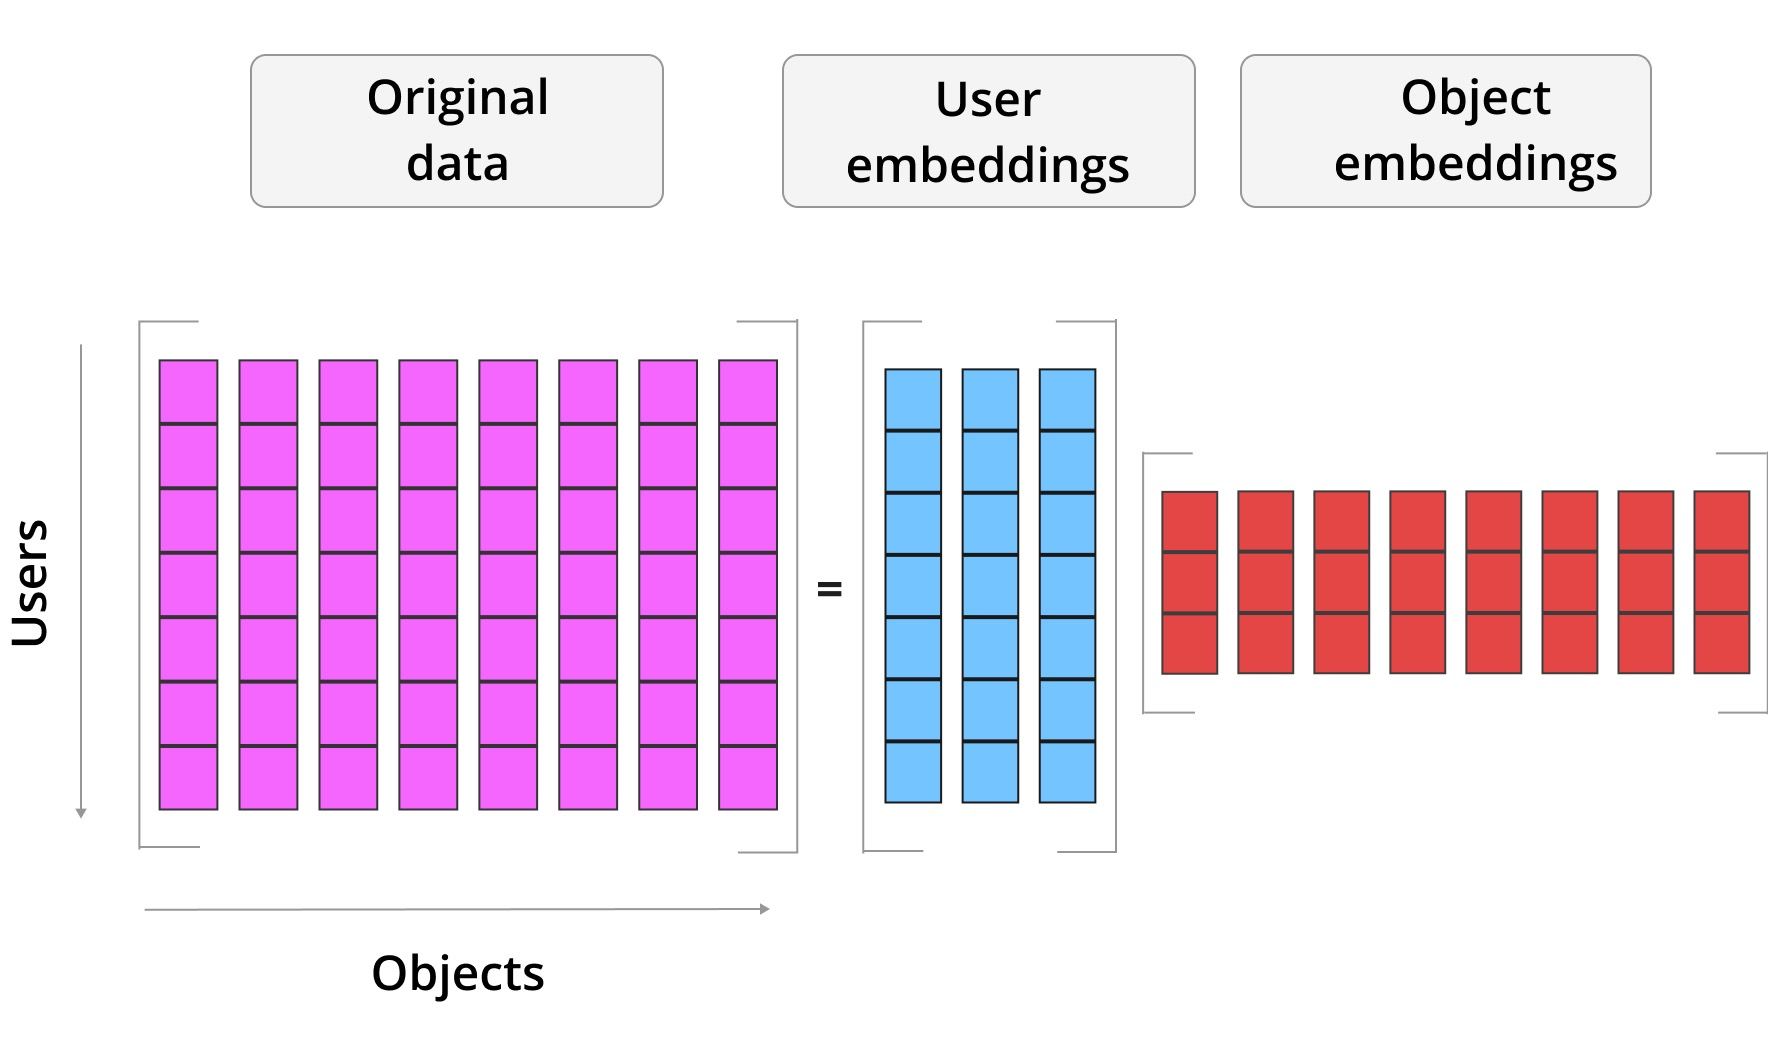
\includegraphics[scale=0.25]{images/mf_idea}}
\caption{}
\label{fig:mf}
\end{figure}

Эмбеддинги можно понимать как вектора скрытых свойств, присущих пользователям и объектам, как правило, обладающие низкой размерностью.
Матрицы, полученные в ходе разложения, являются матрицами эмбеддингов.

Задача разложения матрицы может быть переформулирована как задача оптимизации с определённой функцией потерь.
Для нахождения разложения матрицы эмбеддингов инициализируются случайными элементами, а далее, путем минимизации ошибки рассчитываются актуальные значения.
В процессе матричного разложения значения в исходной матрице аппроксимируются значениями реконструированной матрицы, разряженность которой снижается, что значит, что мы получаем значения для неизвестных (нулевых) элементов исходной матрицы.
Предсказанная оценка для пары пользователь-объект суть произведение соответствующих векторов матриц разложения.

\vspace{1em}
\textbf{Alternating Least Squares (ALS)}


Зададим предсказанную оценку как произведение векторов, соответствующих пользователю и объекту:
\begin{equation}\label{eq:1}
    \hat{r_{ui}} = U_{u} \cdot V_{i},
\end{equation}
где $U_{u}, V_{i}$ --- вектора скрытых признаков пользователя и объекта соответственно.

Тогда функция потерь может быть задана следующим образом:
\begin{equation}\label{eq:2}
        L = \sum_{u, i\in S}{(r_{ui} - U_{u} \cdot V_{i}) ^ 2},
\end{equation}
где $S$ --- множество пар пользователей/объектов, с которыми производилось взаимодействие.

Для защиты от переобучения используется L2-регуляризация~\cite{l-reg}:
\begin{equation}\label{eq:3}
        L = \sum_{u, i\in S}{(r_{ui} - U_{u} \cdot V_{i}) ^ 2} + \lambda_{U}\sum_{u}{\|U_{u}\| ^ 2} + \lambda_{V}\sum_{i}{\|V_{i}\| ^ 2},
\end{equation}
где $\lambda_{U}, \lambda_{V}$ --- гиперпараметры модели для регуляризации.


Метод предполагает минимизацию ошибки путём последовательного фиксирования одного набора векторов скрытых признаков и обновления другого.
Дифференцируя отдельно по признакам пользователей, отдельно по признакам объектов, получают выражения для производной:

\begin{equation}\label{eq:4}
        \frac{\partial L}{\partial U_{u}} = -2\sum_{i}{(r_{ui} - U_{u} \cdot V_{i})V_{i} + 2 \lambda_{U}U_{u}}
\end{equation}

\begin{equation}\label{eq:5}
        \frac{\partial L}{\partial V_{i}} = -2\sum_{u}{(r_{ui} - U_{u} \cdot V_{i})U_{i} + 2 \lambda_{V}V_{i}}
\end{equation}

Приравнивая производную к нулю, получают выражения для искомых векторов:
\begin{equation}\label{eq:6}
        U_{u} = r_{u}V(V^\intercal V + \lambda_{U} E)^{-1}
\end{equation}

\begin{equation}\label{eq:7}
        V_{i} = r_{i}U(U^\intercal U + \lambda_{V} E)^{-1}
\end{equation}

Выбрав размерность эмбеддингов и параметры регуляризации, итеративно рассчитывая новые значения целиком сначала для одного набора векторов, а затем для другого, вычисляют матрицы разложений.


\vspace{1em}
\textbf{Stochastic Gradient Descent (SGD)}

Оценки разных пользователей описываются разными распределениями, то же верно и для объектов взаимодействия.
Чтобы учесть это, в модель добавляют поправку на центр распределения.

Тогда предсказанная оценка представляется следующим образом:
\begin{equation}\label{eq:8}
    \hat{r_{ui}} = \mu + \mu_u + \mu_i+ U_{u} \cdot V_{i},
\end{equation}
где $U_{u}, V_{i}$ --- вектора скрытых признаков пользователя и объекта соответственно,
$\mu, \mu_u, \mu_i$ --- общее среднее, среднее пользователя и среднее объекта соответственно.


Функция потерь с L2-регуляризацией:
\begin{equation}\label{eq:9}
        L = \sum_{u, i\in S}{(r_{ui} - \hat{r_{ui}})) ^ 2} + \lambda_{U}\sum_{u}{(\|U_{u}\| ^ 2 + \|\mu_{u}\| ^ 2)} + \lambda_{V}\sum_{i}{(\|V_{i}\| ^ 2 + \|\mu_{i}\| ^ 2)},
\end{equation}
где $S$ --- множество пар пользователей/объектов, с которыми производилось взаимодействие.

Минимизация производится посредством стохастического градиентного спуска.
Значения градиентов по переменным:

\begin{equation}\label{eq:10}
        \frac{\partial L}{\partial U_{u}} = -2\sum_{i}{(r_{ui} - \hat{r_{ui}})V_{i} + 2 \lambda_{U}U_{u}}
\end{equation}

\begin{equation}\label{eq:11}
        \frac{\partial L}{\partial V_{i}} = -2\sum_{u}{(r_{ui} - \hat{r_{ui}})U_{i} + 2 \lambda_{V}V_{i}}
\end{equation}

\begin{equation}\label{eq:12}
        \frac{\partial L}{\partial \mu_{u}} = -2\sum_{i}{(r_{ui} - \hat{r_{ui}}) + 2 \lambda_{U}\mu_{u}}
\end{equation}

\begin{equation}\label{eq:13}
        \frac{\partial L}{\partial \mu_{i}} = -2\sum_{u}{(r_{ui} - \hat{r_{ui}}) + 2 \lambda_{V}\mu_{i}}
\end{equation}

На каждой итерации вектора обновляются на основе градиента ошибки, который рассчитывается для одной или, если обучение ведётся батчами, нескольких пар оценок.
Таким образом уравнения для обновления векторов признаков записываются как:

\begin{equation}\label{eq:14}
        U_{u} = U_{i} + \nu ((r_{ui} - \hat{r_{ui}})V_{i} - \lambda_{U}U_{i})
\end{equation}
\begin{equation}\label{eq:15}
        V_{i} = V_{i} + \nu ((r_{ui} - \hat{r_{ui}})U_{u} - \lambda_{V}V_{i})
\end{equation}
\begin{equation}\label{eq:16}
        \mu_{u} = \mu_{u} + \nu (r_{ui} - \hat{r_{ui}} - \lambda_{U}\mu_{u})
\end{equation}
\begin{equation}\label{eq:17}
        \mu_{i} = \mu_{i} + \nu (r_{ui} - \hat{r_{ui}} - \lambda_{V}\mu_{i})
\end{equation}
где $\nu$ --- коэффициент скорости обучения.

Выбрав размерность эмбеддингов, параметры регуляризации и скорость обучения, итеративно вычисляют матрицы разложений.

\vspace{1em}
\textbf{Probabilistic Matrix Factorization (PMF)}

Следующий подход был предложен в ~\cite{pmf}.
Идея строится на Байесовском выводе.
Предполагается, что множество оценок нормально распределено относительно предсказанных оценок с общей дисперсией:
\begin{equation}\label{eq:ratings-distr}
        p(R|U, V, \sigma^2) = \prod_{u, i \in S}{N(r_{ui}|U_{u}V_{i}, \sigma^2)},
\end{equation}
где $S$ --- множество пар пользователей/объектов, с которыми производилось взаимодействие,
$N$ --- нормальное распределение.\\
Предполагается, что:
\begin{itemize}
\item Оценки независимы;
\item Оценки нормально распределены с дисперсией $\sigma^2$.
\end{itemize}
Распределения векторов признаков задаётся распределением Гаусса с центром в нуле:

\begin{equation}\label{eq:features-distr}
\begin{aligned}
        p(U|\sigma_{U}^2) = \prod_{u}{N(U_{u}|0, \sigma_{U}^2)} \\
        p(V|\sigma_{V}^2) = \prod_{i}{N(V_{i}|0, \sigma_{V}^2)}
\end{aligned}
\end{equation}
Предполагается, что:
\begin{itemize}
\item Вектора пользователей и объектов независимы между собой;
\item Вектора пользователей и объектов нормально распределены с дисперсией $\sigma^2$.
\end{itemize}
Задав априорные распределения, можно перейти к апостериорному выводу.
Исходя из правила Байеса:
\begin{equation}\label{eq:21}
        p(U,V|R, \sigma^2) = \frac{p(R|U, V, \sigma^2)p(U,V|\sigma^2)}{p(R|\sigma^2)} \propto p(R|U, V, \sigma^2)p(U,V|\sigma^2)
\end{equation}
Так как вектора признаков независимы, можно переписать выражение:
\begin{equation}\label{eq:aposteriori-probs}
        p(U,V|R, \sigma^2) = p(R|U, V, \sigma^2)p(U|\sigma_{U}^2)p(V|\sigma_{V}^2)
\end{equation}
С учётом \eqref{eq:ratings-distr} и \eqref{eq:features-distr}:
\begin{equation}\label{eq:aposteriori-inferred}
        p(U,V|R, \sigma^2) = \prod_{u, i \in S}{N(r_{ui}|U_{u}V_{i}, \sigma^2)} \prod_{u}{N(U_{u}|0, \sigma_{U}^2)} \prod_{i}{N(V_{i}|0, \sigma_{V}^2)}
\end{equation}
Максимизация этой функции эквивалентна максимизации логарифмированного её варианта:
\begin{equation}\label{eq:aposteriori-inferred}
        ln~p(U,V|R, \sigma^2) = - \frac{1}{2\sigma^2}\sum_{u, i \in S}{(r_{ui} - U_{u}V_{i})^2} - \frac{1}{2\sigma_{U}^2}\sum_{u}{\|U_{u}\|^2} - \frac{1}{2\sigma_{V}^2}\sum_{i}{\|V_{i}\|^2}
\end{equation}
Таким образом функция потерь представляется в знакомом виде:
\begin{equation}\label{eq:aposteriori-inferred}
        L = \frac{1}{2}(\sum_{u, i \in S}{(r_{ui} - U_{u}V_{i})^2} - \lambda_{U}\sum_{u}{\|U_{u}\|^2} - \lambda_{V}\sum_{i}{\|V_{i}\|^2})
\end{equation}
где $\lambda_{U} = \frac{\sigma^2}{\sigma_{U}^2}$,
$\lambda_{V} = \frac{\sigma^2}{\sigma_{V}^2}$.

\vspace{0.5em}
Особенность PMF заключается в возможности пересчёта параметров регуляризации на каждой итерации, что позволяет вносить новую информацию в модель по мере обучения.
Для вычисления матриц разложения можно применить ALS или SGD подходы, рассмотренные ранее.

\pagebreak
\paragraph{Нейронные сети для рекомендаций}

Подход с использованием нейронных сетей можно рассматривать как модификацию подхода с использованием матричного разложения.
Идея для обучения нейронной сети основывается на том факте, что матрицы эмбеддингов, получаемые в ходе разложения матриц, могут быть смоделированы нейросетью.
Для этого используется один из слоёв сети, в качестве параметров которого выступают случайным образом инициализированные эмбеддинги.
Параметры этого слоя передаются на вход последующим слоям нейросети и в процессе обучения изменяются таким образом, чтобы давать корректные значения оценок для пар пользователей и объектов.
На рисунке~\ref{fig:nn_idea} приведена схема использования нейросетей для решения описанной задачи:
%В процессе обучения нейронная сеть самостоятельно выучивает эмбеддинги для пар пользователей и объектов так, чтобы эти пары давали корректные значения оценок.

\begin{figure}[h!]
\center{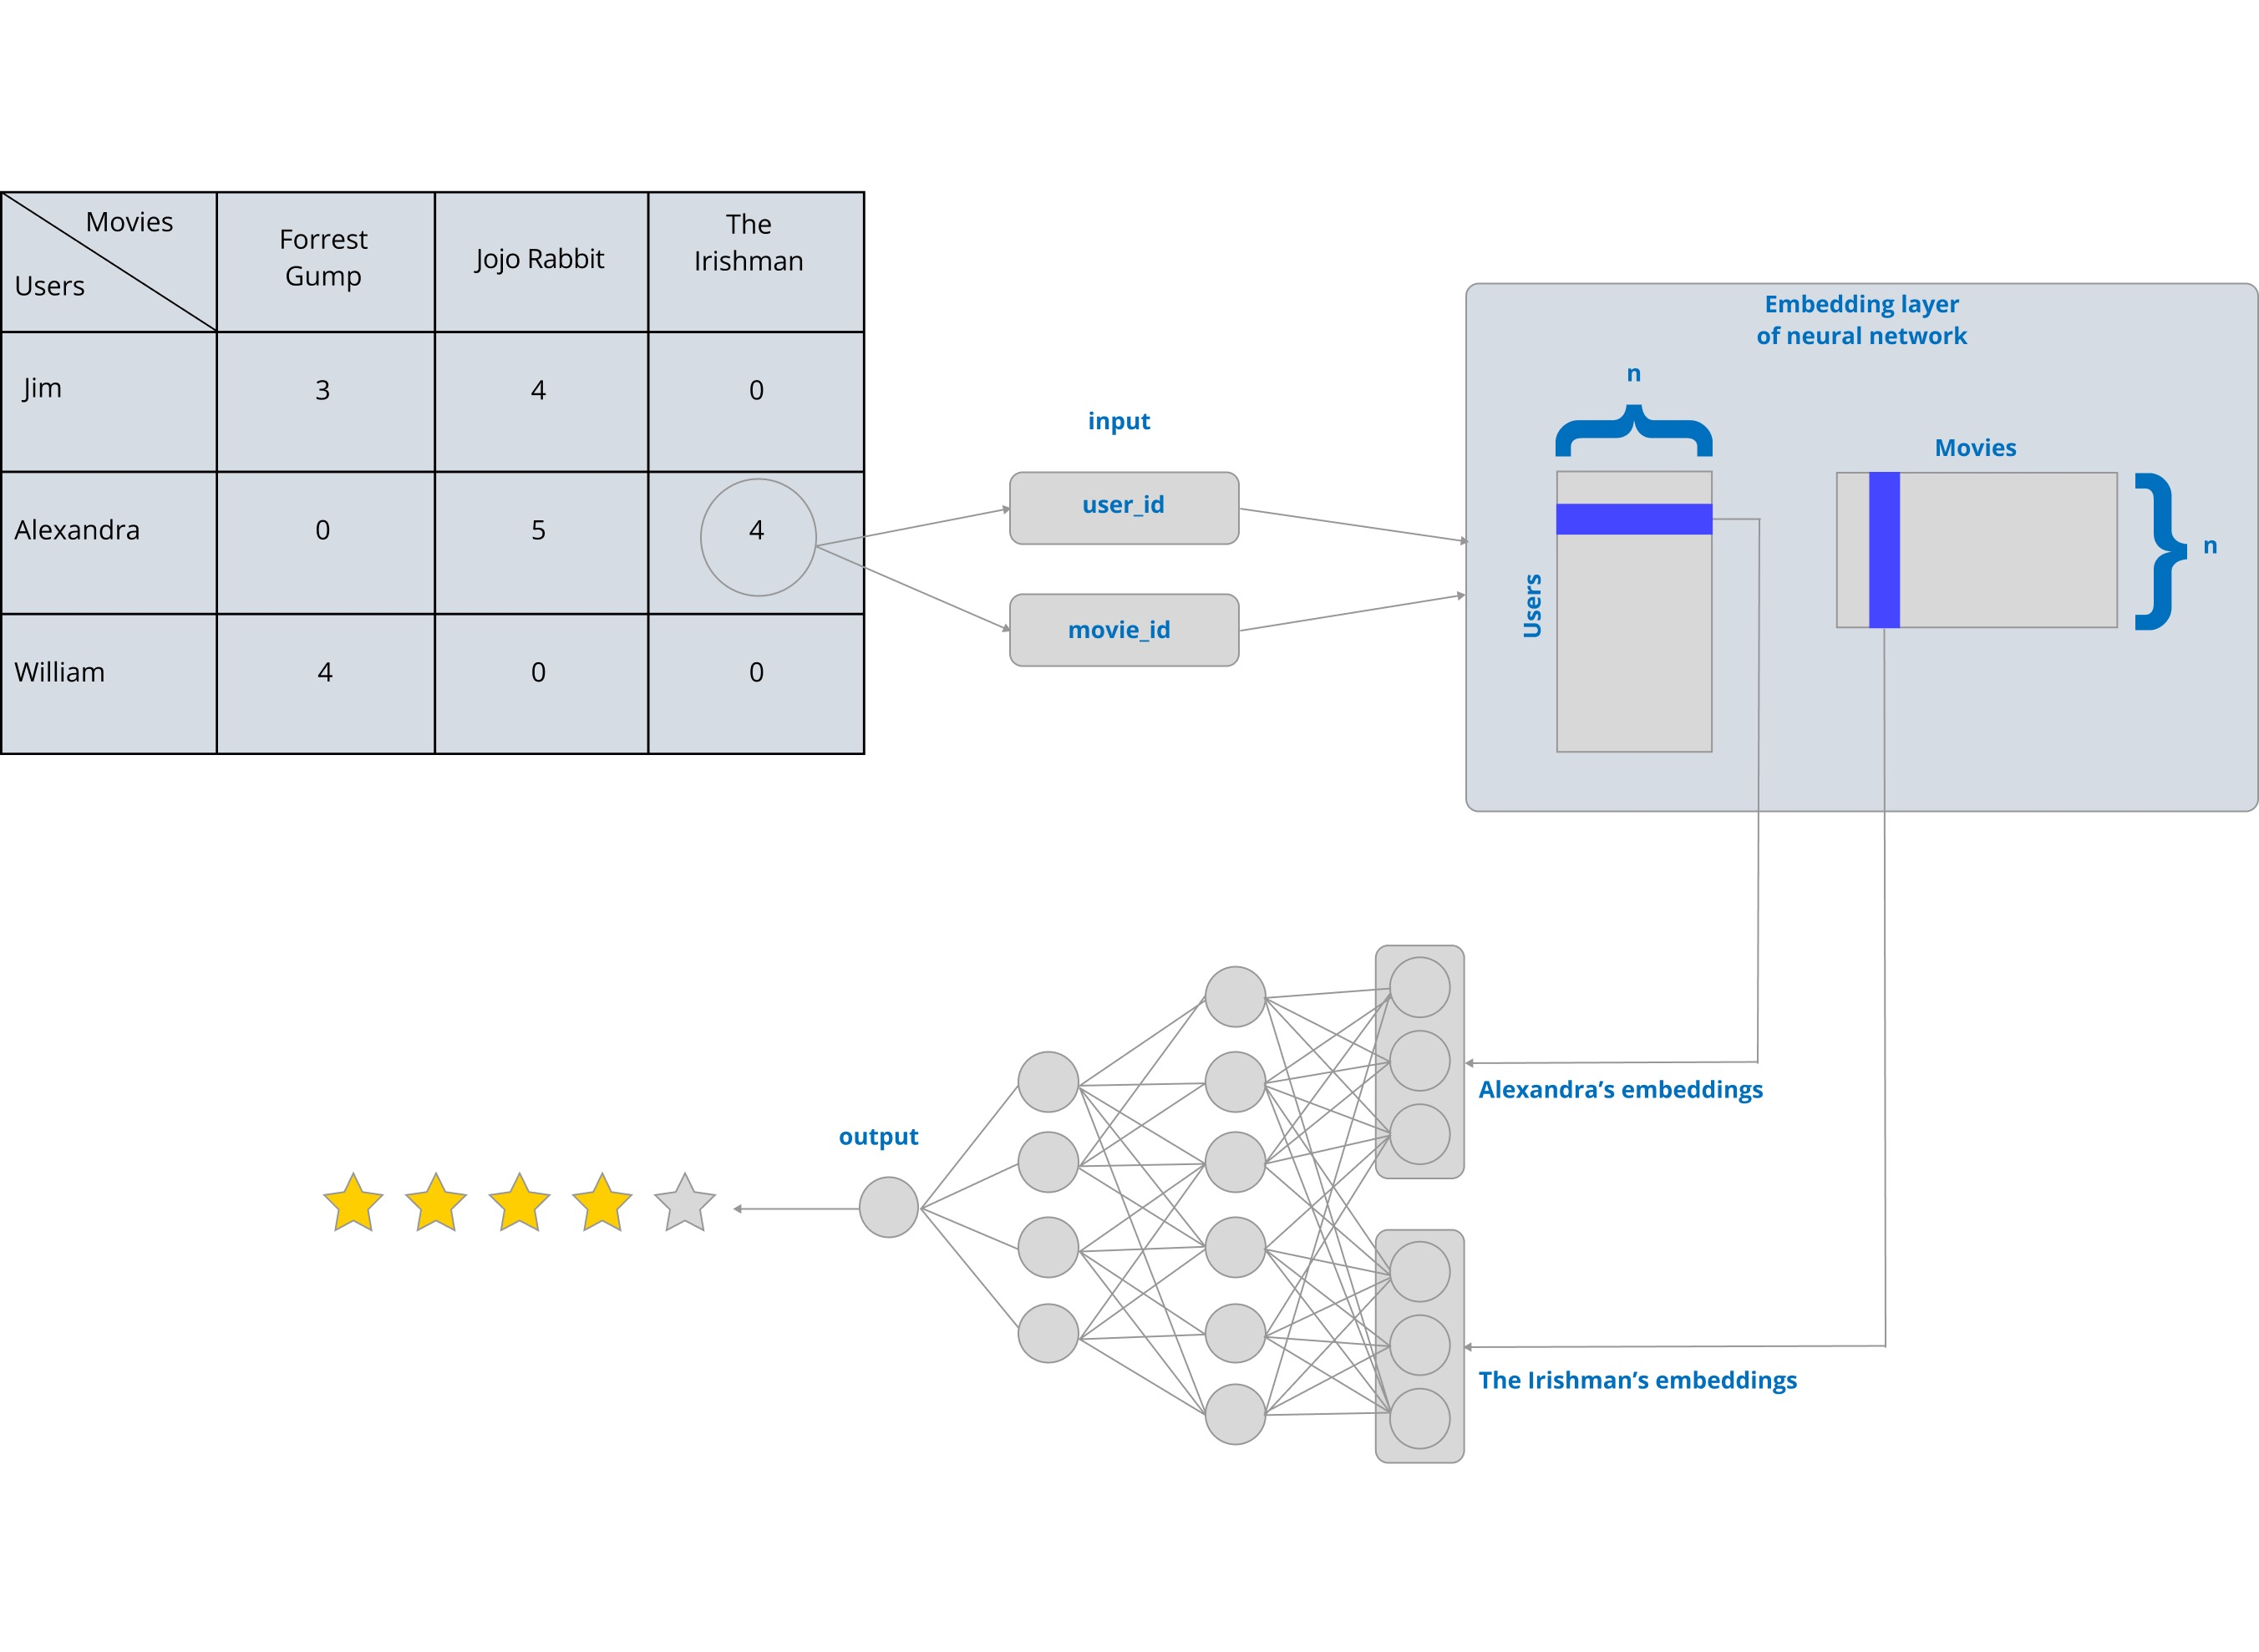
\includegraphics[scale=0.14]{images/nn_idea}}
\caption{}
\label{fig:nn_idea}
\end{figure}

\pagebreak
\subsection{Рекомендательные системы на основе содержимого}\label{subsec:content_rec_systems}
Техники коллаборативной фильтрации обладают существенным минусом --- для них актуальна проблема "холодного старта".
У новых объектов отсутствует история взаимодействий, в следствие чего модель не рекомендует их пользователям, и не происходит накопление информации.
Как правило, у объектов, с которыми взаимодествуют пользователи, можно заранее выделить некоторые признаки.
Это может быть год выхода, режиссёр, актёрский состав фильма; цена или категория товара.
На основе подобных признаков работают \textbf{content-based} алгоритмы.
\\Машинные алгоритмы не могут напрямую работать с нечисловыми признаками, такими как тэги фильма.
Чтобы получить числовое представление таких признаков, можно использовать \textbf{TF-IDF}~\cite{tfidf} (TF — term frequency, IDF — inverse document frequency).
Объекты представляются в виде документов, в которые включаются все словесные признаки.
Ниже приведены формулы, по которым вычисляется TF-IDF мера.
\\\textbf{TF} --- отношение числа вхождений некоторого слова к общему числу слов документа:
\begin{equation}\label{eq:tf}
        tf(t, d) = \frac{n_{t}}{\sum_{k}{n_{k}}},
\end{equation}
где $n_{k}$ --- число вхождений слова $k$ в документ $d$.
\\\textbf{IDF} --- инвертированная частота, с которым слово встречается в корпусе:
\begin{equation}\label{eq:idf}
        idf(t, D) = log~\frac{\|D\|}{\|\{d_{i} \in D \| t \in d_{i}\}\|},
\end{equation}
где $D$ --- множество документов в корпусе.
\\Мера \textbf{TF-IDF}:
\begin{equation}\label{eq:tf-idf}
        tf\textnormal{-}idf(t, d, D) = tf(t, d) \times idf(t, D)
\end{equation}

Но такое представление фрагментированно и избыточно, так как каждому слову будет соответствовать отдельное измерение, и вектора, соответствующие синонимичным словам, будут ортогональны.
Чтобы сжать пространство можно использовать автоэнкодеры~\cite{autoencoders} --- специальные нейросети, обученные предсказывать то же, что получили на вход.
Архитектура автоэнкодера представлена на рисунке~\ref{fig:autoencoder_simple}:

\begin{figure}[h!]
\center{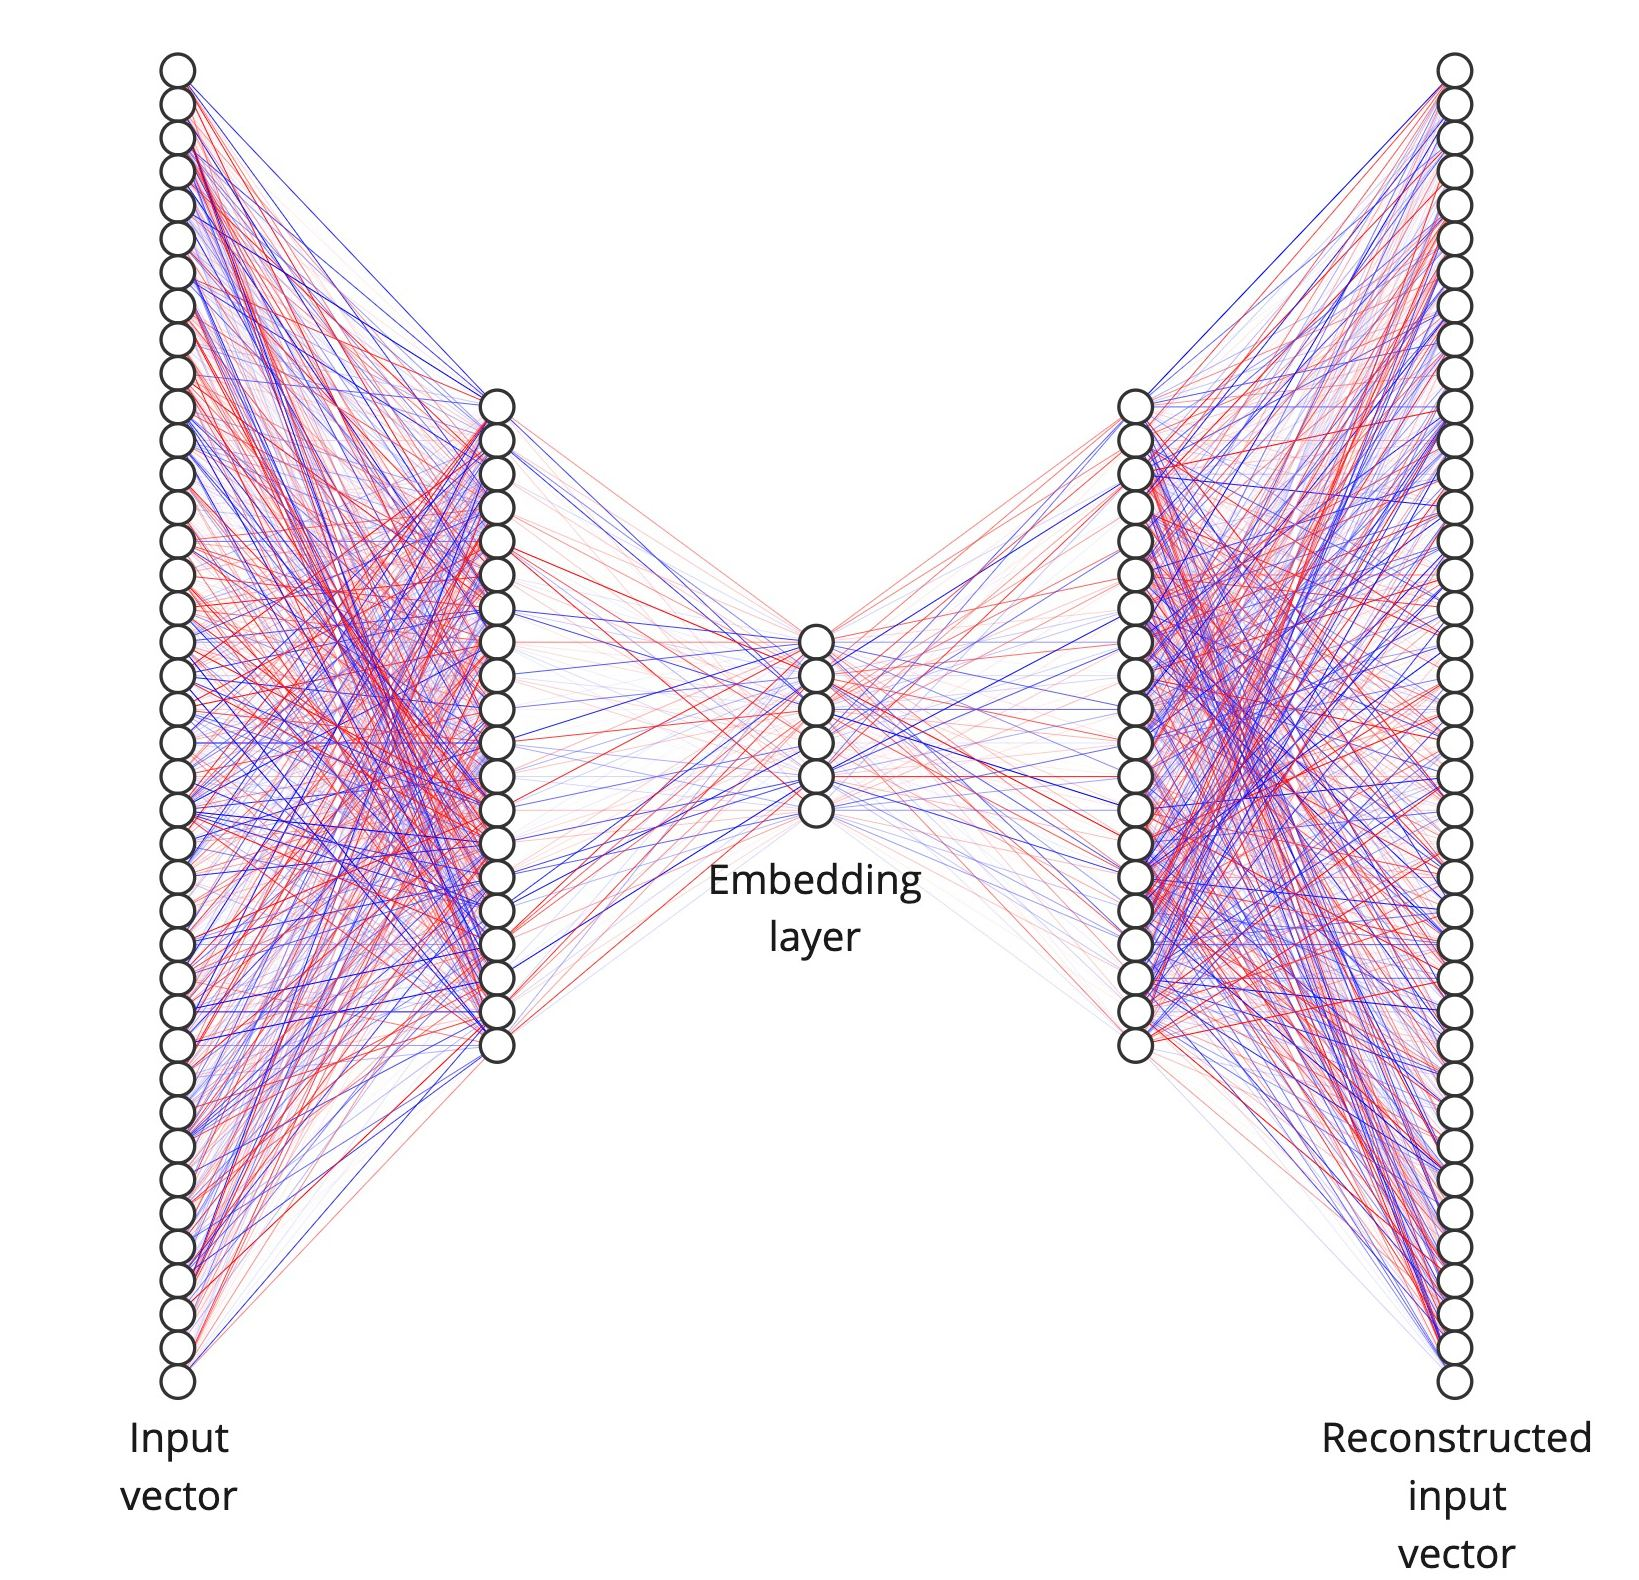
\includegraphics[scale=0.25]{images/autoencoder_simple}}
\caption{}
\label{fig:autoencoder_simple}
\end{figure}

Данная архитектура сжимает многомерное TF-IDF пространство в n-мерное.
Первая половина сети (энкодер) кодирует вектор, соответствующий объекту, а вторая половина (декодер) реконструирует оригинальные данные.
Сжатое представление в n-мерном пространстве моделируется центральным слоем сети.

Полученные таким образом векторные представления объектов дают возможность включать в рекомендации объекты, не имеющие истории взаимодействия.
Мы можем дополнительно получить вектор пользователя в пространстве, порождённым автоэнкодером, взяв взвешенную сумму векторов объектов, с которыми тот уже взаимодействовал:
\begin{equation}\label{eq:content-user-emb}
        U_{i}^{c} = \sum_{j \in S_i}{R_{ij}~I_{j}^{c}},
\end{equation}
где $S_i$ --- множество объектов, с которыми взаимодействовал пользователь $i$,
$R$ --- матрица оценок,
$U^c$, $I^c$ --- матрицы эмбеддингов пользователей и объектов.

Тогда релевантность объекта $j$ для пользователя $i$ может быть вычислена с помощью косинусного сходства:
\begin{equation}\label{eq:content-user-rel}
    \begin{aligned}
        & rel_{ij} = 0.5~\frac{U_{i}^{c} \cdot I_{j}^{c}}{\| U_{i}^{c} \| \| I_{j}^{c} \|} + 0.5, \\
        & rel_{ij} \in [0, 1]
    \end{aligned}
\end{equation}

Соответственно, предсказанная оценка:
\begin{equation}\label{eq:content-user-rating}
        \hat{R_{ij}} = r_{\min} + (r_{\max} - r_{\min}) rel_{ij},
\end{equation}
где $r_{\min}$, $r_{\max}$ --- минимально и максимально возможные оценки.

Кроме того, есть возможность рекомендовать похожие между собой объекты, вычисляя похожесть через косинусное сходство.
\pagebreak

\subsection{Гибридные рекомендательные системы}\label{subsec:hybrid_rec_systems}
Гибридная модель сочетает в себе коллаборативные модели с контентными, используя знания обеих для улучшения качества ранжирования рекомендуемых пользователю объектов.
Для этого коллаборативная модель решает какие $n$ объектов являются релевантными по отношению к пользовательскому запросу.
Затем контентная модель самостоятельно задаёт порядок ранжирования или вносит в него поправки, используя свои знания о релевантности объектов.

Однако, также можно выделить ещё две задачи, которые может решить гибридная рекомендательная система:
\begin{enumerate}
    \item Рекомендация объектов, похожих на заинтересовавший пользователя объект.
    \item Рекомендация объектов, похожих на заинтересовавший пользователя объект, с учётом предпочтений пользователя.
\end{enumerate}

\noindentДля решения также предполагается двухэтапное ранжирование.

\noindentЗадача 1:
\begin{addmargin}[2em]{1em}% 1em left, 2em right
Контентная модель задаёт порядок ранжирования по схожести с объектом интереса и отбирает $n$ самых близких.
\end{addmargin}

\noindentЗадача 2:
\begin{addmargin}[2em]{1em}% 1em left, 2em right
Контентная модель отбирает $n$ похожих объектов, а коллаборативная модель сортирует их с учётом весов, присвоенных объектам контентной моделью, или без.
\end{addmargin}

\vspace{1em}
И коллаборативная, и контентная модели обладают возможностью самостоятельно задавать релевантность объекта для пользователя, их решения можно совмещать.
Тогда ранжирование с учётом весов присвоенных обеими моделями математически выражается так:
\begin{equation}\label{eq:hybrid}
rel_{ij} = (1 - \alpha)\space M_1(i, j) + \alpha\space M_2(i, j)
\end{equation}
Выбирая $\alpha$, можно менять вклад модели в конечную оценку.
